\documentclass[sigconf]{acmart}

\usepackage{amsmath}
\usepackage{algorithm}
\usepackage[noend]{algpseudocode}
\usepackage{tikz}
\usepackage{pgfplots}

\graphicspath{ {images/} }

\setcopyright{none}
\acmConference[ICPP'19]{ICPP 2019}{August 2019}{Kyoto, Japan}
\acmYear{2019}
\copyrightyear{2019}

\begin{document}
	
	\title{Fractional Eigenbasis Compression Placeholder Title}
	
	\author{<Author 1>}
	\affiliation{%
		\institution{<Institution 1>}
		\city{<City 1>}
		\state{<State 1>}
	}
	\email{<E-mail 1>}
	
	\author{<Author 2>}
	\affiliation{%
		\institution{<Institution 1>}
		\city{<City 1>}
		\state{<State 1>}
	}
	\email{<E-mail 2>}
	
	\author{<Author 3>}
	\affiliation{%
		\institution{<Institution 1>}
		\city{<City 1>}
		\state{<State 1>}
	}
	\email{<E-mail 3>}
	
	\begin{abstract}
		In order to study the non-local diffusion operator known as the fractional laplacian, we have developed a framework to solve a simple fractional poisson problem using the spectral expansion method. This framework requires computation of a set of eigenpairs for the given problem geometry. For analytical purposes, we compute the entire eigenbasis in order to explore the impact of the non-local nature of the fractional laplacian on the convergence of the spectral expansion. Additionally, we employ the zfp compression library to reduce the amount of data required to store the full eigenbasis. Using this compression library, we explore strategies for balancing data reduction and performance impact in addition to leveraging any aspect of the non-local operator to improve either data reduction or performance.
		
		{\color{blue} This abstract will be updated as results are put into the paper. "We will explore" statements will be replaced with more concrete statements about results.}
	\end{abstract}
	
	\maketitle
	
	\section{Introduction}
	{\color{green} \noindent <Project motivation> }

{\color{blue} \noindent <Introduce fractional operators> }

{\color{red} \noindent <Introduce Nektar++> }

{\color{blue} \noindent <Introduce SLEPc> }

{\color{blue} \noindent <Introduce zfp> }
	
	\section{Fractional Laplacian}
	{\color{blue} \noindent <Define fractional poisson problem> }

{\color{blue} \noindent <Define spectral approach to solving fractional poisson problem> }

{\color{blue} \noindent <Describe non-local nature of fractional properties and what aspects can and can not be captured by the spectral approach> }
	
	\section{Eigenbasis Computation}
	In order to compute solutions to our fractional model problem, the method of eigenfunction expansion requires the computation of the discrete eigenbasis for a given geometry. Since scalability is the primary computational concern for this framework, we build our framework on top of PETSc \cite{petsc-efficient} \cite{petsc-user-ref} and SLEPc \cite{slepc}. PETSc is a parallel and scalable library of routines and data structures for scientific applications. PETSc handles how our matrices are stored in parallel and for operations like matrix multiplication. 

Since our framework is built in the method of eigenfunction expansion, we build on top of the SLEPc library for solving the resulting eigenvalue problem. SLEPc has a number of routines available for solving eigenvalue problems and is also built on PETSc. Our approach requires computing the full set of eigenpairs for a system and therefore our framework uses a modified version of spectrum slicing with the independent eigenvalue problems being solved with SLEPc.

{\color{red} \noindent <Introduce Nektar++, expand nektar++ integration description, cite \cite{nektarpp}> }

\subsection{Method}

In order to construct solutions to the fractional poisson problem, we need to discretize the domain of interest. Using the finite element method, geometry can be converted into the symmetric, discrete system $ Kv_k = \lambda_k M v_k $. For this, we have integerated our framework with Nektar++ which is used to convert a given mesh into two PETSc matrices $K$ and $M$.

Equipped with these matrices, we can compute all of the eigenpairs in a given interval using SLEPc's Krylov-Schur solver. Krylov-Schur is an iterative solver that relies on applying $K$ and $M$ repeatedly and solving related systems. If we were to simply give $K$ and $M$ to SLEPc, these sparse  matrices would be divided among the entire set of available processes. Using this naive approach, throwing more processes at the problem will just result in more communication between nodes and will hurt performance. Instead, we use an approach to split the full eigenbasis computation into independent subproblems that can be handled by a single node. This results in a much more scalable approach.

\subsubsection{Spectrum Slicing}

In order to compute the full set of eigenpairs using the available computing resources, we use the method of spectrum slicing. Because we know the eigenvalue problem is symmetric, all of the eigenvalues are real, and because the problem is semidefinite, all of the eigenvalues are contained in the interval $[0,U]$. Instead of solving for all eigenpairs within this interval using all processes, we break it into independent subintervals that can be solved in parallel. This is possible, again, due to the symmetry of the problem. 

For a symmetric system, if any two eigenvectors have different eigenvalues, they are inherently orthogonal. Therefore any eigenvectors that are in separate subintervals can be solved for independently without any need for orthogonalization between subintervals.

Each subinterval is solved by a group of processes we refer to as an evaluator. Each evaluator is comprised of a number of nodes that is determined based on problem size and then each node is broken up into its component processes. This communication hierarchy ensures that each evaluator's system is spread out across as few nodes as possible, resulting in minimal communication when applying the discretized operators.

For this approach, we then needed some method for breaking the interval into subintervals that require equal amounts of work to solve. If we were to instead assume that the eigenvalues are equally distributed and then split the interval evenly among evaluators, very bad load imbalance occurs. The worst case of this load imbalance occurs using this naive splitting with two evaluators. For a simple cube domain, the lower half of the interval contains the vast majority of eigenvalues, and therefore the second evaluator has almost no work to do.

One potential way of making this assumption of uniformly distributed eigenvalues work as a splitting method is to split the interval into a large number of subintervals per evaluator and then distribute them in a round-robin fashion. This approach does reduce the load imbalance to some extent but isn't reliable. We did end up using some ideas from this, specifically having many subintervals per evaluator distributed in a round-robin fashion. This idea was helpful so that no single evaluator had all of their subintervals in a region that is very sparse.

\subsubsection{Counting an Interval}

In order to count how many eigenvalues are contained in an interval [a,b], there are two techniques that we explored. Both approaches are based on counting the number of eigenvalues greater than $a$ and then the number greater than $b$ and taking the difference to get the interval count. 

Given some matrix $A$ that can be factored such that $A = LDL^T$, where L is a lower triangular matrix and D is a diagonal matrix, the Sylvester inertia theorem states that the inertia of $D$ and $A$ are the same. This means that the number of entries of $D$ that are greater than 0 is also the number of eigenvalues of $A$ that are greater than 0. Therefore if we let $A$ be the shifted eigenvalue problem centered around $a$, specifically that $A = K - aM$, we can compute this factorization to get the number of eigenvalues greater than some given value of $a$.

While this method results in very accurate eigenvalue counts, it becomes prohibitively expensive as the size of the problem increases. Therefore an approximate counting technique was required to find a balance between accuracy and scaling complexity. For this, we use a method called polynomial expansion filtering. 

This approach, which is outline in full detail in \cite{eigcount}, relies on two separate approximations that are composed together. The first bit of machinery is that of approximating the trace of a matrix using $n_v$ random vectors. Specifically, this approximation can be seen in equation \eqref{eq:trace}.

\begin{equation}
\label{eq:trace}
\text{tr}(A) \approx \frac{1}{n_v} \sum_{k=1}^{n_v} v_k^TAv_k
\end{equation}

The approximate count of eigenvalues in an interval is computed by approximating the trace of the eigenprojector of $A$, which is referred to as $P$. The second bit of machinery is that of approximating this eigenproject $P$ by polynomial expansion filtering as seen in equation \eqref{eq:polyfilter}. By plugging the matrix $A$ into the chebyshev expansion of degree $p$ of the heaviside function centered at 0, an approximate form of $P$ is constructed.

\begin{equation}
\label{eq:polyfilter}
	P \approx \phi_p(A) = \sum_{j=0}^{p} \gamma_j T_j(A)
\end{equation}

For the generalized eigenvalue problem we are attempting to solve, the count of eigenvalues in an interval $[a,b]$ is then the difference of the counts for the two shifted systems $K-aM$ and $K-bM$. Specifically, this can be seen in equation \eqref{eq:eigapprox}.

\begin{equation}
\label{eq:eigapprox}
	\mu_{[a,b]} = \mu_a - \mu_b \approx \text{tr}[\phi_p (K-aM) - \phi_p (K-bM)]
\end{equation}

\subsection{Results}

One of the main assumptions that determine the load balancing of the spectrum slicing approach is that if two independent subintervals have an equal number of eigenvalues, that they take equal amounts of time to solve. Some of the early experiments with the approximate eigenvalue counting technique resulted in very uneven distribution of eigenvalues per subinterval. However, using the data from these experiments, we plotted each subinterval's solve time and eigenvalue count and can be seen in figure \ref{fig:solvetime_vs_count}. From this it can be seen there is a very distinct linear relationship between the eigenvalue count and solve time.

\begin{figure}
	\caption{Comparison of number of eigenvalues within a subinterval and the amount of time taken to solve for all eigenpairs within the subinterval. Observe the clear linear relationship between the two values.}
	\label{fig:solvetime_vs_count}
	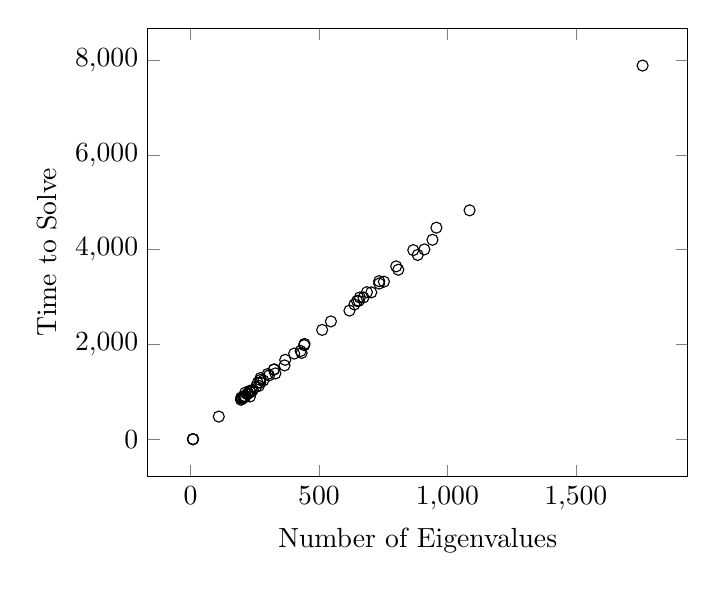
\begin{tikzpicture}
\begin{axis}[scatter/classes={a={mark=o,draw=black}}, xlabel=Number of Eigenvalues, ylabel=Time to Solve,]
\addplot[scatter, only marks, scatter src=explicit symbolic]
table[meta=label] {
x y label
239.2956240000000037 1021 a
330.3349410000000148 1388 a
403.5728119999999990 1807 a
428.7328989999999749 1862 a
196.3786660000000097 831 a
212.6695799999999963 892 a
271.6221679999999878 1249 a
271.6146870000000035 1194 a
324.1807329999999752 1468 a
212.8577870000000019 981 a
212.3631880000000081 906 a
546.5748539999999593 2486 a
209.4923919999999953 897 a
205.6613969999999938 876 a
201.3032220000000052 855 a
197.2036870000000022 879 a
206.6175869999999861 903 a
220.0788949999999886 951 a
208.5720809999999972 894 a
224.0978100000000097 966 a
230.0824330000000089 1020 a
242.3957100000000082 1039 a
255.5193179999999984 1107 a
283.4893969999999968 1239 a
261.4792969999999741 1189 a
272.4084330000000023 1290 a
365.9100129999999922 1557 a
325.5648630000000026 1474 a
368.6733070000000225 1674 a
512.5255150000000413 2307 a
1760.1893569999999727 7887 a
443.5480269999999905 2011 a
232.9014530000000036 991 a
637.9793929999999591 2844 a
199.2110230000000115 856 a
206.2969300000000032 883 a
673.4450839999999516 2991 a
654.8509609999999839 2919 a
231.2846040000000016 900 a
659.2124089999999796 2992 a
265.9438599999999724 1125 a
686.7583969999999454 3103 a
734.5700640000000021 3285 a
300.1143059999999991 1374 a
752.9143199999999752 3325 a
432.5287599999999770 1821 a
808.9818960000000061 3577 a
800.6906579999999849 3648 a
648.1655130000000327 2917 a
884.5558039999999664 3889 a
941.9991619999999557 4209 a
957.2640509999999949 4465 a
703.7453389999999445 3099 a
442.6263839999999732 1985 a
10.0058849999999993 0 a
1086.5890220000001136 4831 a
618.8599239999999782 2714 a
9.2223360000000003 0 a
734.5807459999999764 3336 a
305.7018360000000143 1346 a
9.1900119999999994 0 a
910.4873229999999467 4006 a
867.2910699999999906 3991 a
109.9918600000000026 477 a
};
\end{axis}
\end{tikzpicture}

\end{figure}

In order to verify that our method results in near-optimal load balancing, we ran the eigenbasis computation for a range of problem sizes and number of evaluators. These experiments were run on the <Institution 1>'s <Cluster 1> computing cluster with 28 processes per node and a single node per evaluator. The results of this scaling experiment can be seen in figure \ref{fig:scaling}.

\begin{figure}
	\caption{The time it takes to compute the full eigenbasis for various problem sizes vs the number of nodes used.}
	\label{fig:scaling}
	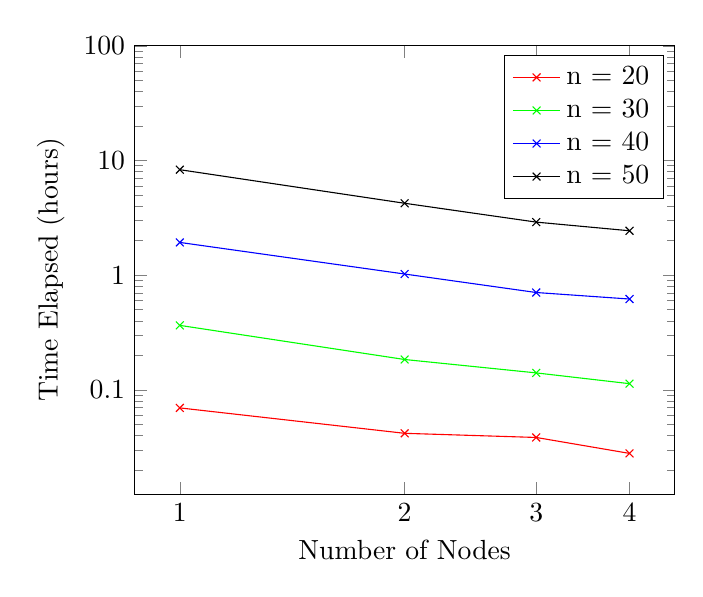
\begin{tikzpicture}
\begin{loglogaxis} [xlabel=Number of Nodes, ylabel=Time Elapsed (hours), log ticks with fixed point, xtick = {1,2,3,4}, ymax = 100]
\addplot[color=red, mark=x] coordinates {
(1, 0.0696913636111111)
(2, 0.0418443866666667)
(3, 0.0385055244444444)
(4, 0.0279569738888889)
};
\addlegendentry{n = 20}\addplot[color=green, mark=x] coordinates {
(1, 0.3653069425000000)
(2, 0.1841394594444444)
(3, 0.1407181208333333)
(4, 0.1133450255555556)
};
\addlegendentry{n = 30}\addplot[color=blue, mark=x] coordinates {
(1, 1.9314824902777779)
(2, 1.0242012847222222)
(3, 0.7066568988888889)
(4, 0.6199479344444444)
};
\addlegendentry{n = 40}\addplot[color=black, mark=x] coordinates {
(1, 8.3164149672222223)
(2, 4.2385486824999994)
(3, 2.9037166197222226)
(4, 2.4406479241666670)
};
\addlegendentry{n = 50}\end{loglogaxis}
\end{tikzpicture}

\end{figure}

Since the total eigenbasis computation is divided into smaller independent tasks, one way to determine load balancing is to observe the scaling efficiency per number of evaluators. For $p$ evaluators, the scaling efficiency is then equal to $t_1 / (p\cdot t_p) $, where $t_1$ is the time elapsed for a single evaluator and $t_p$ is the maximum time elapsed for all of the $p$ evaluators. The closer this value is to 1, the closer the work is divided perfectly evenly among evaluators. Ideally, this value should be 1 or close to it. The resulting scaling efficiency can then be seen in figure \ref{fig:efficiency}.

\begin{figure}
	\caption{Scaling efficiency vs problem size with respect to number of nodes.}
	\label{fig:efficiency}
	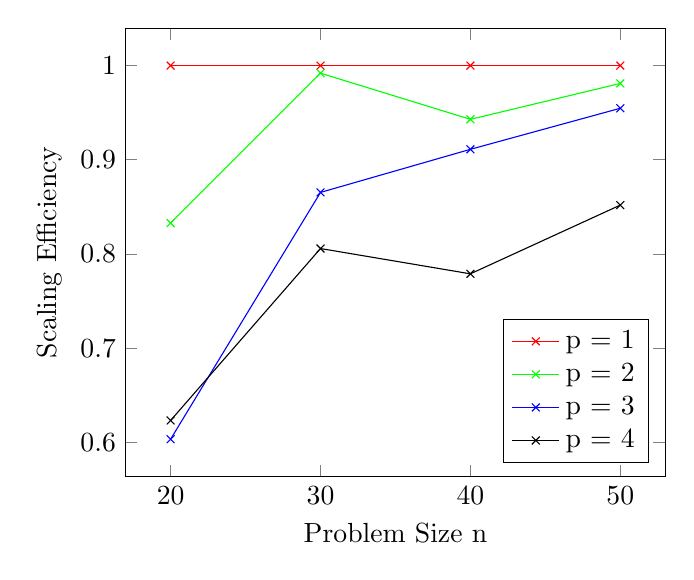
\begin{tikzpicture}
\begin{axis} [xlabel=Problem Size n, ylabel=Scaling Efficiency, xtick = {1, 2, 3, 4}, xticklabels = {20,30,40,50}, ytick = {0.6, 0.7, 0.8, 0.9, 1.0}, legend pos = south east]
\addplot[color=red, mark=x] coordinates {
(1, 1.0000000000000000)
(2, 1.0000000000000000)
(3, 1.0000000000000000)
(4, 1.0000000000000000)
};
\addlegendentry{p = 1}\addplot[color=green, mark=x] coordinates {
(1, 0.8327444749790944)
(2, 0.9919300936424615)
(3, 0.9429213373822428)
(4, 0.9810451159330554)
};
\addlegendentry{p = 2}\addplot[color=blue, mark=x] coordinates {
(1, 0.6033018605045571)
(2, 0.8653397310326268)
(3, 0.9110892397308801)
(4, 0.9546862471285500)
};
\addlegendentry{p = 3}\addplot[color=black, mark=x] coordinates {
(1, 0.6232019592686404)
(2, 0.8057410122532163)
(3, 0.7788889933187060)
(4, 0.8518654908062756)
};
\addlegendentry{p = 4}\end{axis}
\end{tikzpicture}

\end{figure}

{\color{blue} \noindent <Comparison of performance and accuracy of exact and approximate interval counting> }

\subsection{Potential Improvements}

Our framework results in close to optimal load balancing for the simple domains we have tested, however, it isn't necessarily guaranteed. We could make better guarantees of the load balancing by designating a single process to maintain a queue of subintervals to be processed. Using this approach, as each evaluator finishes a subinterval, it can report to the task manager and request the next subinterval. This way, the only time any evaluator is starved for work is when there is no more work to be done. 

Since the newest versions of PETSc have incorporated GPU acceleration, we could then set up GPU evaluators alongside the previously mentioned CPU evaluators. In this case, a task queue would be essential to properly manage the work among the different types of evaluators. Even if the GPU evaluators are not faster than the CPU evaluators, they would be able to function in parallel, thus resulting in an effective evaluator count greater than the actual number of machines available.
	
	\section{Eigenbasis Storage and Compression}
	{\color{blue} <Details about zfp compression> }

\subsection{Method}

{\color{blue} <Describe Eigenbasis data structure and the available storage modes> }

{\color{blue} <Explain that each storage mode also corresponds to a compression strategy> }

{\color{blue} <Describe how the Eigenbasis is applied and truncation criteria> }

\subsection{Results}

{\color{blue} <Compare compression strategies; Data reduction and time to compress/decompress> }

	
	\section{Results}
	{\color{blue} <Present results relating to the performance of applying the Eigenbasis using the various compression and storage strategies> }

{\color{blue} <Present results relating to the accuracy of spectral approach with various truncation criteria> }
	
	\section{Conclusion}
	In conclusion, we have developed an early version of a scalable framework for computing approximate solutions to fractional PDEs and presented some results for some simple geometries. This is the first step towards more interesting solvers based on the method of eigenfunction expansion. 

In addition to computing the eigenbasis in a scalable, efficient manner, we have laid the groundwork for a compression scheme that will both reduce the amount of data required for such a method as well as reducing the amount of work for applying the eigenbasis. While zfp didn't give quite the results we would prefer, the next step would be to explore geometry-aware compression schemes along the lines of FMM. One of the benefits of such a scheme would be that the geometry doesn't change on an eigenvector by eigenvector basis, any of the geometry-related data structures would only need to be computed once for the mesh. In addition to this, a data structure for compressing and decompressing eigenvectors as needed would need to be developed and tested.

While the eigenbasis computation is in a scalable and efficient state, without GPU acceleration and a task manager, we are leaving computing resources on the table so to speak. Further development on this framework will need to include these features in order to achieve peak efficiency on heterogeneous computing nodes.

Looking ahead, we hope to explore more complicated fractional PDEs such as space-fractional Diffusion-Reaction or Cahn-Hiliard. This framework will act as the foundation for these explorations and should allow for very large-scale experiments to be done to verify existing and future theoretical work in this field.
	
	\bibliographystyle{unsrt}
	\bibliography{refs}
	
\end{document}